    \documentclass[10pt, compress]{beamer}
    
    \usetheme{glasgow}
    
    \usepackage{booktabs}
    \usepackage[scale=2]{ccicons}
    \usepackage{minted}
    \usepackage{bookmark}
    \usepgfplotslibrary{dateplot}
    
    \usemintedstyle{trac}
    
    % ($ (A)!r!(B) $) the location of images to be used
    \graphicspath{{src/}}
    
    %% Customisation
    % \newcommand{\V}[1]{\v} % vectors \v{c}
    % \renewcommand{\v}[1]{\mathbf{#1}} % vectors
    \newcommand{\ti}[1]{\tilde{#1}} % spectral representation
    \newcommand{\tnsr}[1]{\underline{\underline{#1}}}
    
    % Symbols
    \renewcommand{\O}{\omega}  % omega
    \newcommand{\E}{\varepsilon}  % epsilon
    \renewcommand{\u}{\mu}  % mu
    \newcommand{\p}{\rho}  % rho
    \newcommand{\x}{\times}  % times
    \renewcommand{\inf}{\infty}  % infinity
    \newcommand{\infint}{\int\limits_{-\inf}^\inf} % integral by R
    \newcommand{\e}{\mathrm{e}} % Straight-up exponential
    \renewcommand{\j}{{j}\mkern1mu} % Straight-up exponential
    \newcommand{\iu}{\mathrm{i}\mkern1mu}
    
    \newcommand\ddfrac[2]{\frac{\displaystyle #1}{\displaystyle #2}}
    
    \title{High Frequency Communication Systems}
    \subtitle{Lecture 5}
    \date{Spring 2022}
    \author{Hasan T Abbas \& Qammer H Abbasi}
    % \institute{}
    
\begin{document}

\maketitle

%%%%%%%%%%%%%%%%%%%%%%%%%%%%%%%%%%%%%%%%%%
%%%%%%%%%%%%%%%%%%%%%%%%%%%%%%%%%%%%%%%%%%
%%%%%%%%%%%%%%%%%%%%%%%%%%%%%%%%%%%%%%%%%%
\begin{frame}[fragile]
    \frametitle{Lecture Outline}
    \begin{outline}[itemize]
        \1 The Smith Chart
        \1 Quarter-wave Transformer (Magic)
        \1 Some Examples - Load matching through stubs
    \end{outline}
\end{frame}
%%%%%%%%%%%%%%%%%%%%%%%%%%%%%%%%%%%%%%%%%%
%%%%%%%%%%%%%%%%%%%%%%%%%%%%%%%%%%%%%%%%%%
%%%%%%%%%%%%%%%%%%%%%%%%%%%%%%%%%%%%%%%%%%

\section{The Smith Chart}


\begin{frame}
    \frametitle{The Smith Chart}
    \begin{figure}[htbp]
        \centering
        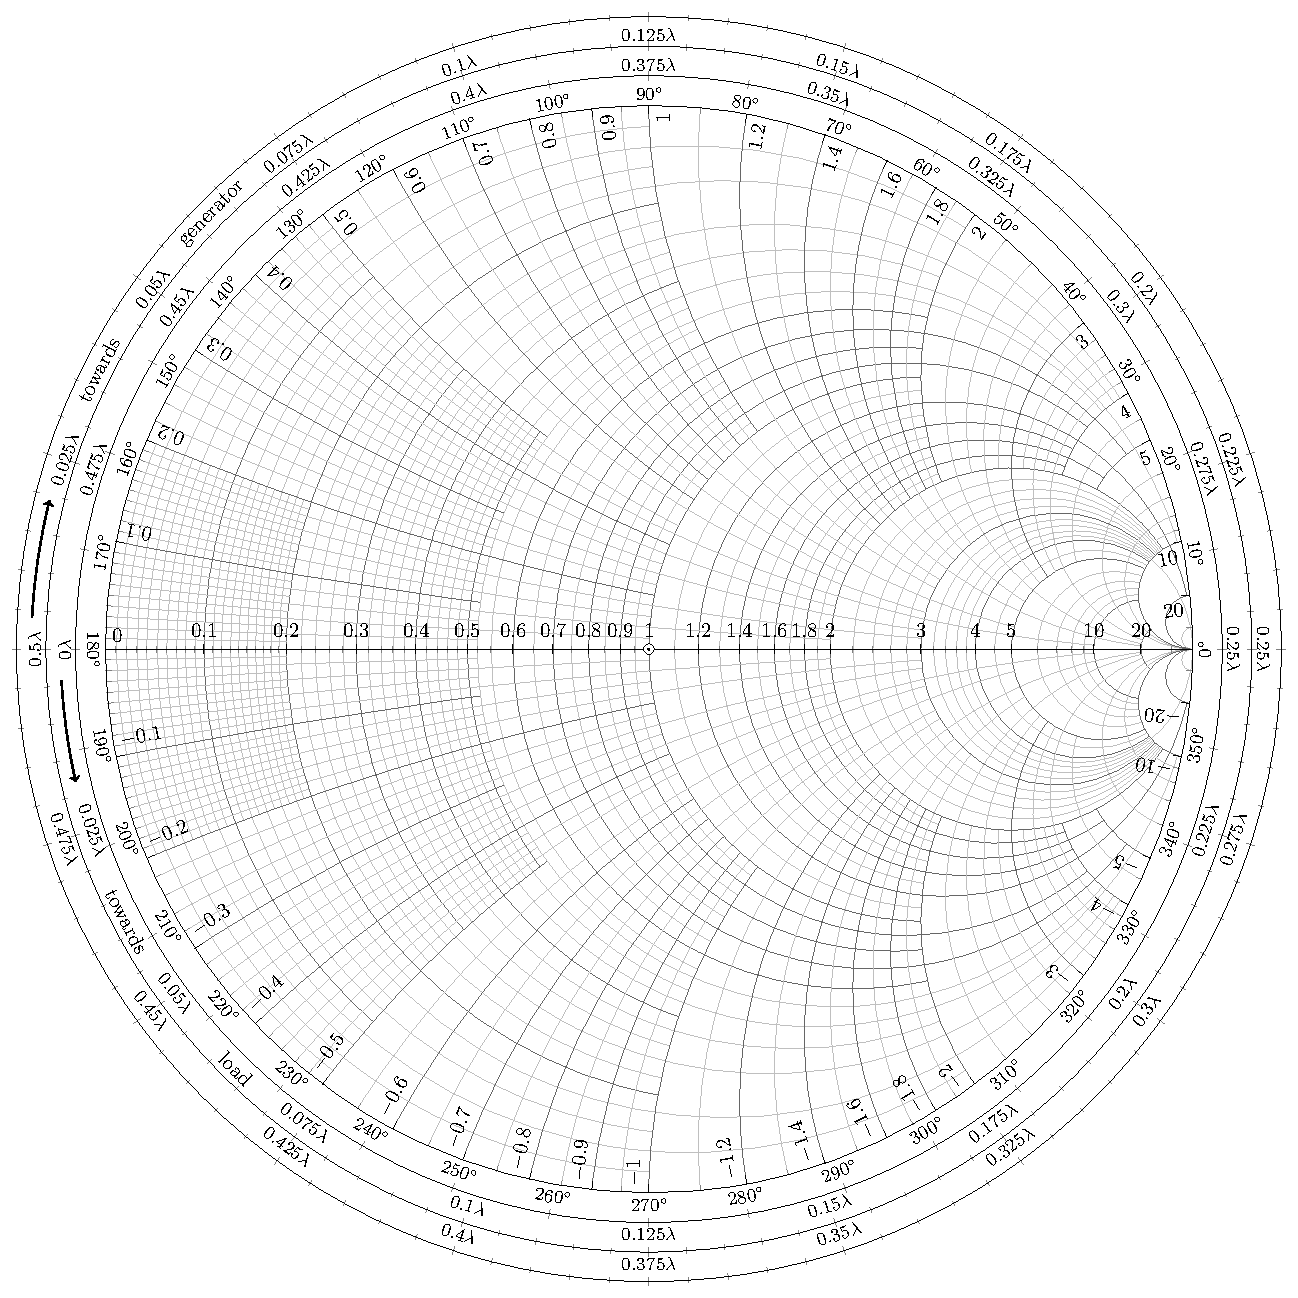
\includegraphics[width=.7\textwidth]{smith.pdf}
    \end{figure}
\end{frame}


\begin{frame}
    \frametitle{Why Smith Chart}
    \begin{outline}
        \1 A nomogram (graphical calculator) invented by Phillip Smith and Mizuhashi Tusaku
        \1 To this day, it is an integral part of microwave circuit design
        \1 Provides a tool to visualise the transmission line phenomena such as impedance matching
        \1 \textcolor{red}{It is simply a polar plot of the reflection coefficient, $\Gamma$}
    \end{outline}
\end{frame}

\begin{frame}
    \frametitle{Navigating the Smith Chart}
    \begin{outline}
        \1 In polar coordinates, $\Gamma = |\Gamma| \e^{\j \theta}$
        \1 We plot the magnitude as a radius $(|\Gamma| \le 1)$ from the centre
        \1 The angle $\theta$ ranges from $\SI{-180}{\degree}$ to $\SI{180}{\degree}$
        \1 \textcolor{red}{The origin} or the centre of the Smith chart is the ideal, matched point.
    \end{outline}
    \begin{figure}[htbp]
        \centering
        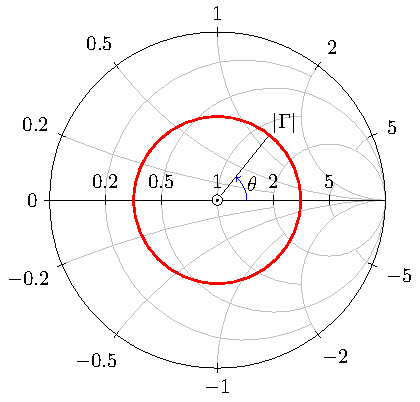
\includegraphics[width=.5\textwidth]{smith_simple_gamme.pdf}
        %   \caption{$\Gamma$ plotted on the Smith chart }
    \end{figure}
\end{frame}

\begin{frame}
    \frametitle{Plotting Impedances}
    For lossless TL's, the \textit{normalised} load impedance at $l = 0$ is a complex number:
    \begin{align*}
        z_L  = \frac{Z_L}{Z_0} & = \frac{1 + |\Gamma|\e^{\j \theta}}{1 - |\Gamma|\e^{\j \theta}}
    \end{align*}
    Treating $\Gamma = \Gamma_r + \j \Gamma_i$, the real and imaginary parts of $z_L$ are:
    \begin{align*}
        r_{L} & = \frac{1-\Gamma_{r}^{2}-\Gamma_{i}^{2}}{\left(1-\Gamma_{r}\right)^{2}+\Gamma_{i}^{2}} \\
        x_{L} & = \frac{2 \Gamma_{i}}{\left(1-\Gamma_{r}\right)^{2}+\Gamma_{i}^{2}}
    \end{align*}
    which can be written as two equations of circles:
    \begin{align*}
        \left(\Gamma_{r} - \frac{r_{L}}{1+r_{L}}\right)^{2} + \Gamma_{i}^{2}      & = \left(\frac{1}{1+r_{L}}\right)^{2} \tag{Resistance Circle} \\
        \left(\Gamma_{r}-1\right)^{2}+\left(\Gamma_{i}-\frac{1}{x_{L}}\right)^{2} & =\left(\frac{1}{x_{L}}\right)^{2} \tag{Reactance Circle}
    \end{align*}
\end{frame}

\begin{frame}
    \frametitle{The Resistance and Reactance Circles}
    \begin{outline}
        \1 Let's look at some examples
        \2 Taking $r_L = 1$ and let's plot in the $\Gamma_r ,\Gamma_i$ plane
        \2 But first, the equation for the resistance circle is:
    \end{outline}
    \begin{align*}
        \left(\Gamma_{r} - \frac{1}{1+1}\right)^{2} + \Gamma_{i}^{2} & = \left(\frac{1}{1+1}\right)^{2}
    \end{align*}
    \begin{figure}[h]
        \centering
        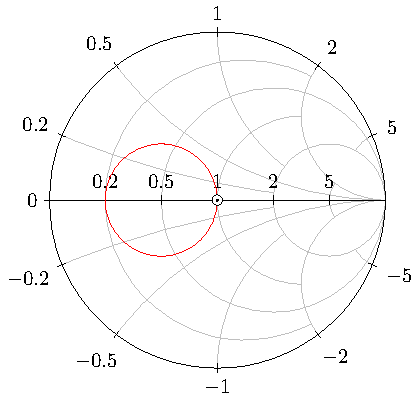
\includegraphics[width=.4\textwidth]{smith_resistance.pdf}
    \end{figure}
\end{frame}

\begin{frame}
    \frametitle{The Resistance and Reactance Circles}

    \begin{outline}
        \1 Now the reactance circle where we take $z_L = \j 1 \implies x_L = 1$
        \1 The reactance circle equation becomes:
    \end{outline}
    \begin{align*}
        \left(\Gamma_{r}-1\right)^{2}+\left(\Gamma_{i}-1\right)^{2} & = 1
    \end{align*}
    \begin{figure}[h]
        \centering
        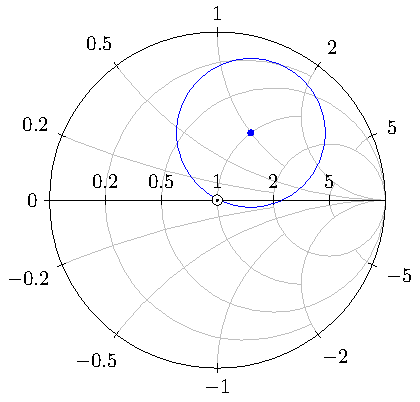
\includegraphics[width=.3\textwidth]{smith_reactance_circle.pdf}
    \end{figure}
    The top half is the \textit{inductive} region and the bottom half is the \textit{capacitive} region.
\end{frame}

\begin{frame}
    \frametitle{Plotting Impedance}
    \begin{columns}[T] % align columns
        \begin{column}{.4\textwidth}
            \begin{outline}
                \1 We normally normalise the impedance to $\SI{50}{\ohm}$.
                \1 However, the chart can be used for any value.
                \1 \textcolor{green}{$z_{L,1} = $ ?}
                \1 \textcolor{red}{$z_{L,2} =  $ ? }
                \1 \textcolor{blue}{$z_{L,3} = $ ? }
                \1 \textcolor{orange}{$z_{L,4} = $ ?}
            \end{outline}
            \begin{figure}
                
\includegraphics[width=.75\textwidth]{QR-code.png}
            \end{figure}
        \end{column}
        \begin{column}[T]{.6\textwidth}
            \begin{figure}
                \centering
                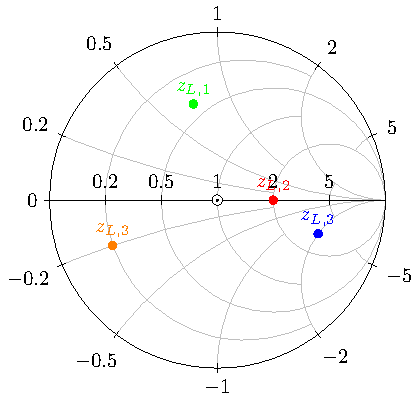
\includegraphics[width=1\textwidth]{smith simple impedances.pdf}
            \end{figure}
        \end{column}%
    \end{columns}
\end{frame}

%% Exercise
\begin{frame}
    \frametitle{Plotting Impedance}
    \begin{columns}[T] % align columns
        \begin{column}{.4\textwidth}
            \begin{outline}
                \1 We normally normalise the impedance to $\SI{50}{\ohm}$.
                \1 However, the chart can be used for any value.
                \1 \textcolor{green}{$z_{L,1} = 0.4 + \j 0.7$}
                \1 \textcolor{red}{$z_{L,2} = 2 $}
                \1 \textcolor{blue}{$z_{L,3} = 3 - \j 2$}
                \1 \textcolor{orange}{$z_{L,4} = 0.2 - \j 0.2$}
            \end{outline}
        \end{column}
        \begin{column}[T]{.6\textwidth}
            \begin{figure}
                \centering
                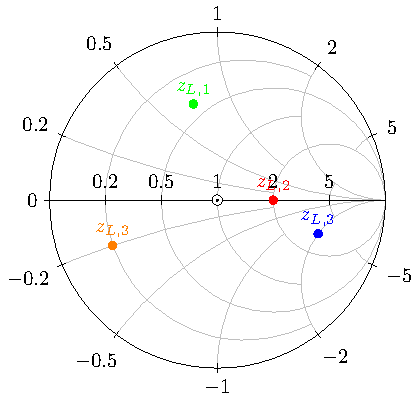
\includegraphics[width=1\textwidth]{smith simple impedances.pdf}
            \end{figure}
        \end{column}%
    \end{columns}
\end{frame}

\begin{frame}
    \begin{figure}[t!]
        \frametitle{Example — Finding the Input Impedance}
        \centering
        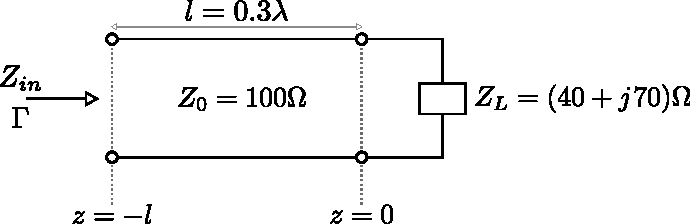
\includegraphics[width=.9\textwidth]{tline_terminated_example.pdf}
    \end{figure}
    \begin{outline}
        \1 Lets find the input impedance $Z_{in} = Z(-l)$ of the line.
        \1 Also the reflection coefficient, $\Gamma$ and the VSWR
    \end{outline}
\end{frame}

\begin{frame}
    \frametitle{Example - Finding the Input Impedance}
    \begin{figure}[T!]
        \centering
        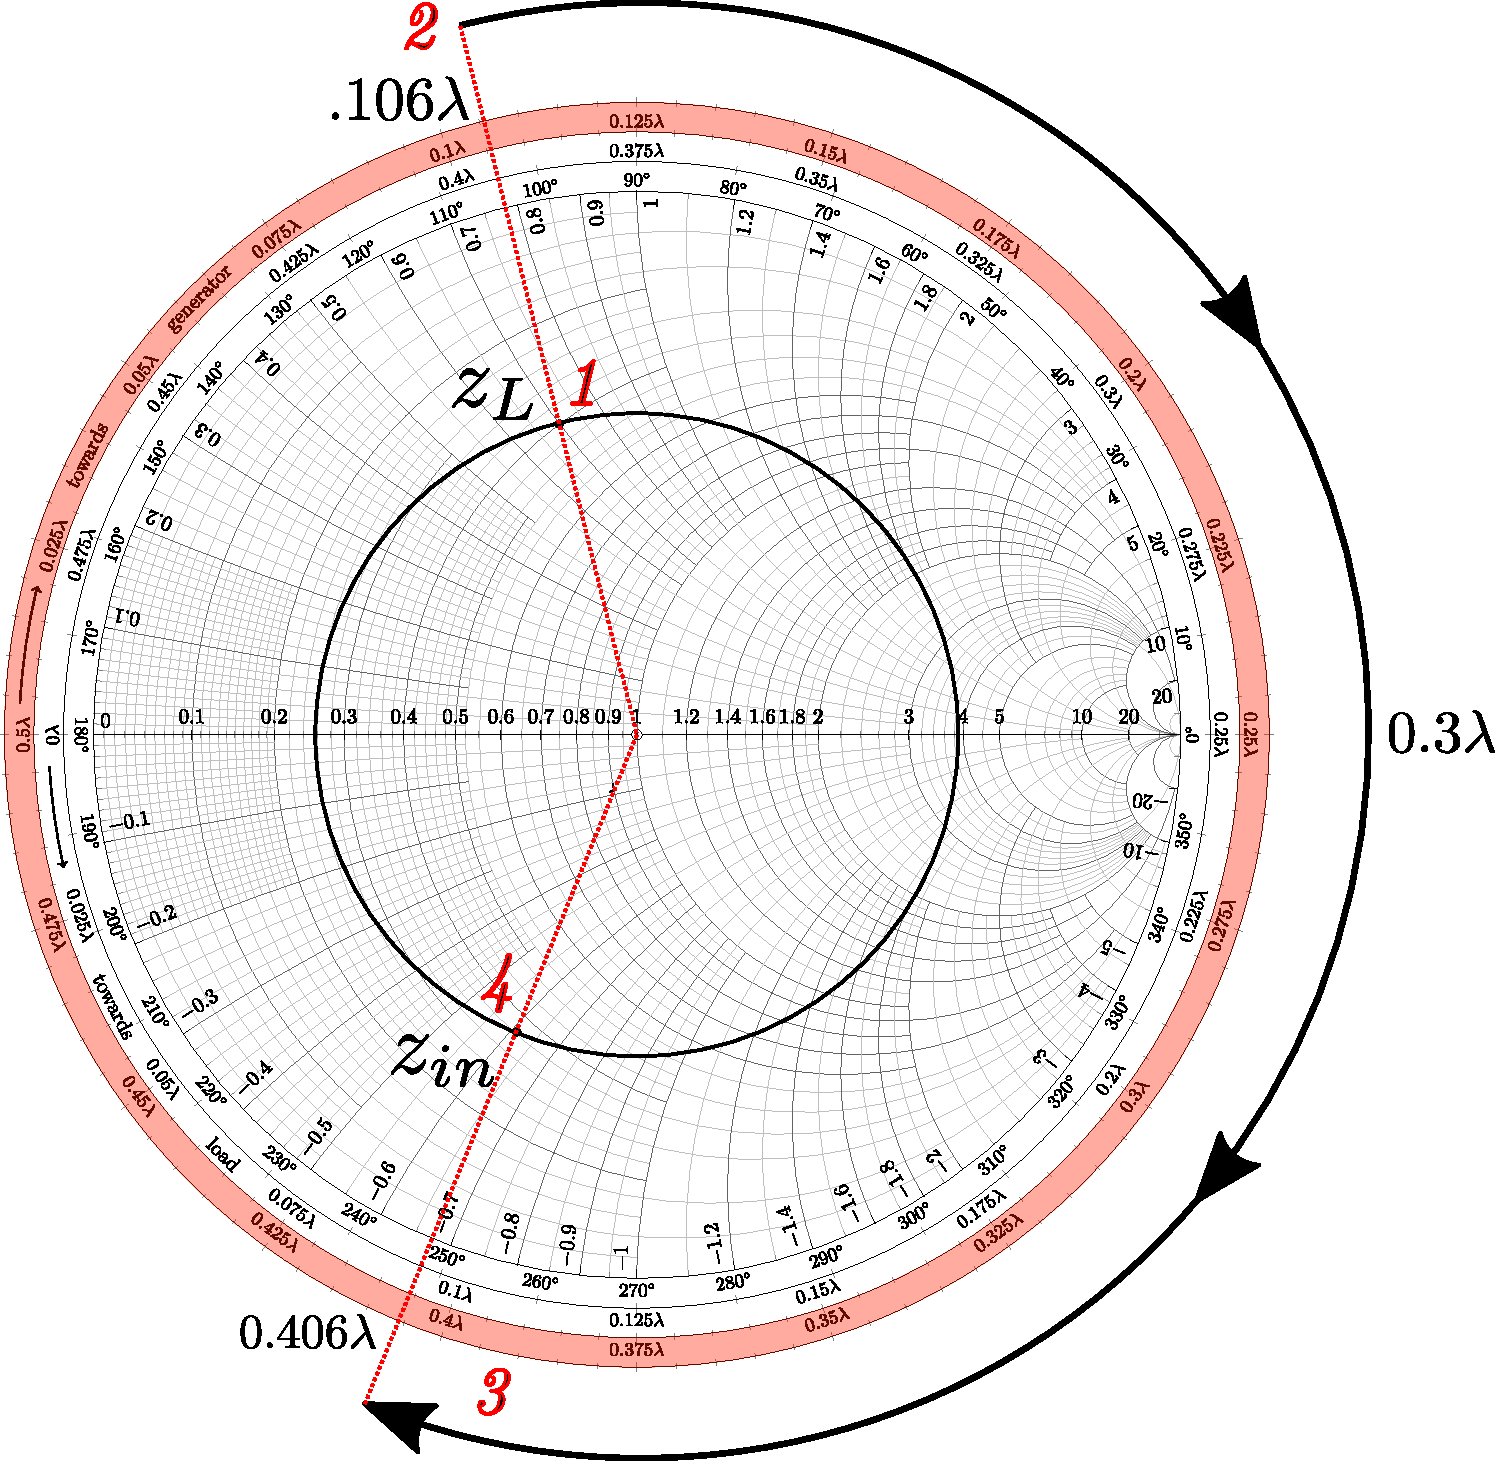
\includegraphics[width=.70\textwidth]{smith example inkspace.pdf}
    \end{figure}

\end{frame}

\begin{frame}
    \frametitle{Finding the Input Impedance}
    \begin{outline}
        \1 From the Smith chart, we first plot the normalised load impedance $z_L$
        \1 We then draw a circle centred on the origin with a radius such that $z_L$ lies on the circle
        \1 Draw a line from the origin passing through $z_L$ to the outer circle of the Smith chart
        \1 Move $l = 0.3 \lambda$ towards the generator
        \1 Draw a line from the origin to the new rotated point.
        \1 The intersection point with the circle and the line drawn gives us the normalised input impedance $z_{in} \approx 0.365 - \j 0.61 $.
    \end{outline}
\end{frame}

\begin{frame}
    \frametitle{Finding the VSWR}
    \begin{figure}[T!]
        \centering
        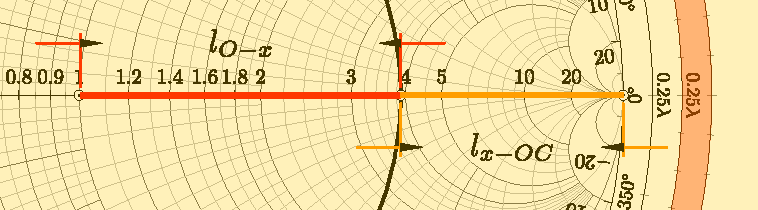
\includegraphics[width=.95\textwidth]{smith example VSWR cropped.pdf}
    \end{figure}
    \begin{outline}
        \1 The ratio of the length of the line segments $l_{O - x}$ and $l_{O - OC}$ gives us VSWR
        \1 The point on the right of the Smith chart is the open-circuit point ($r = \infty, x = \infty$)
        \1 For this example, we get VSWR $\approx 3.9$.
    \end{outline}

\end{frame}

\begin{frame}
    \frametitle{Finding the VSWR — Using the Radially Scaled Parameters}
    \begin{figure}[T!]
        \centering
        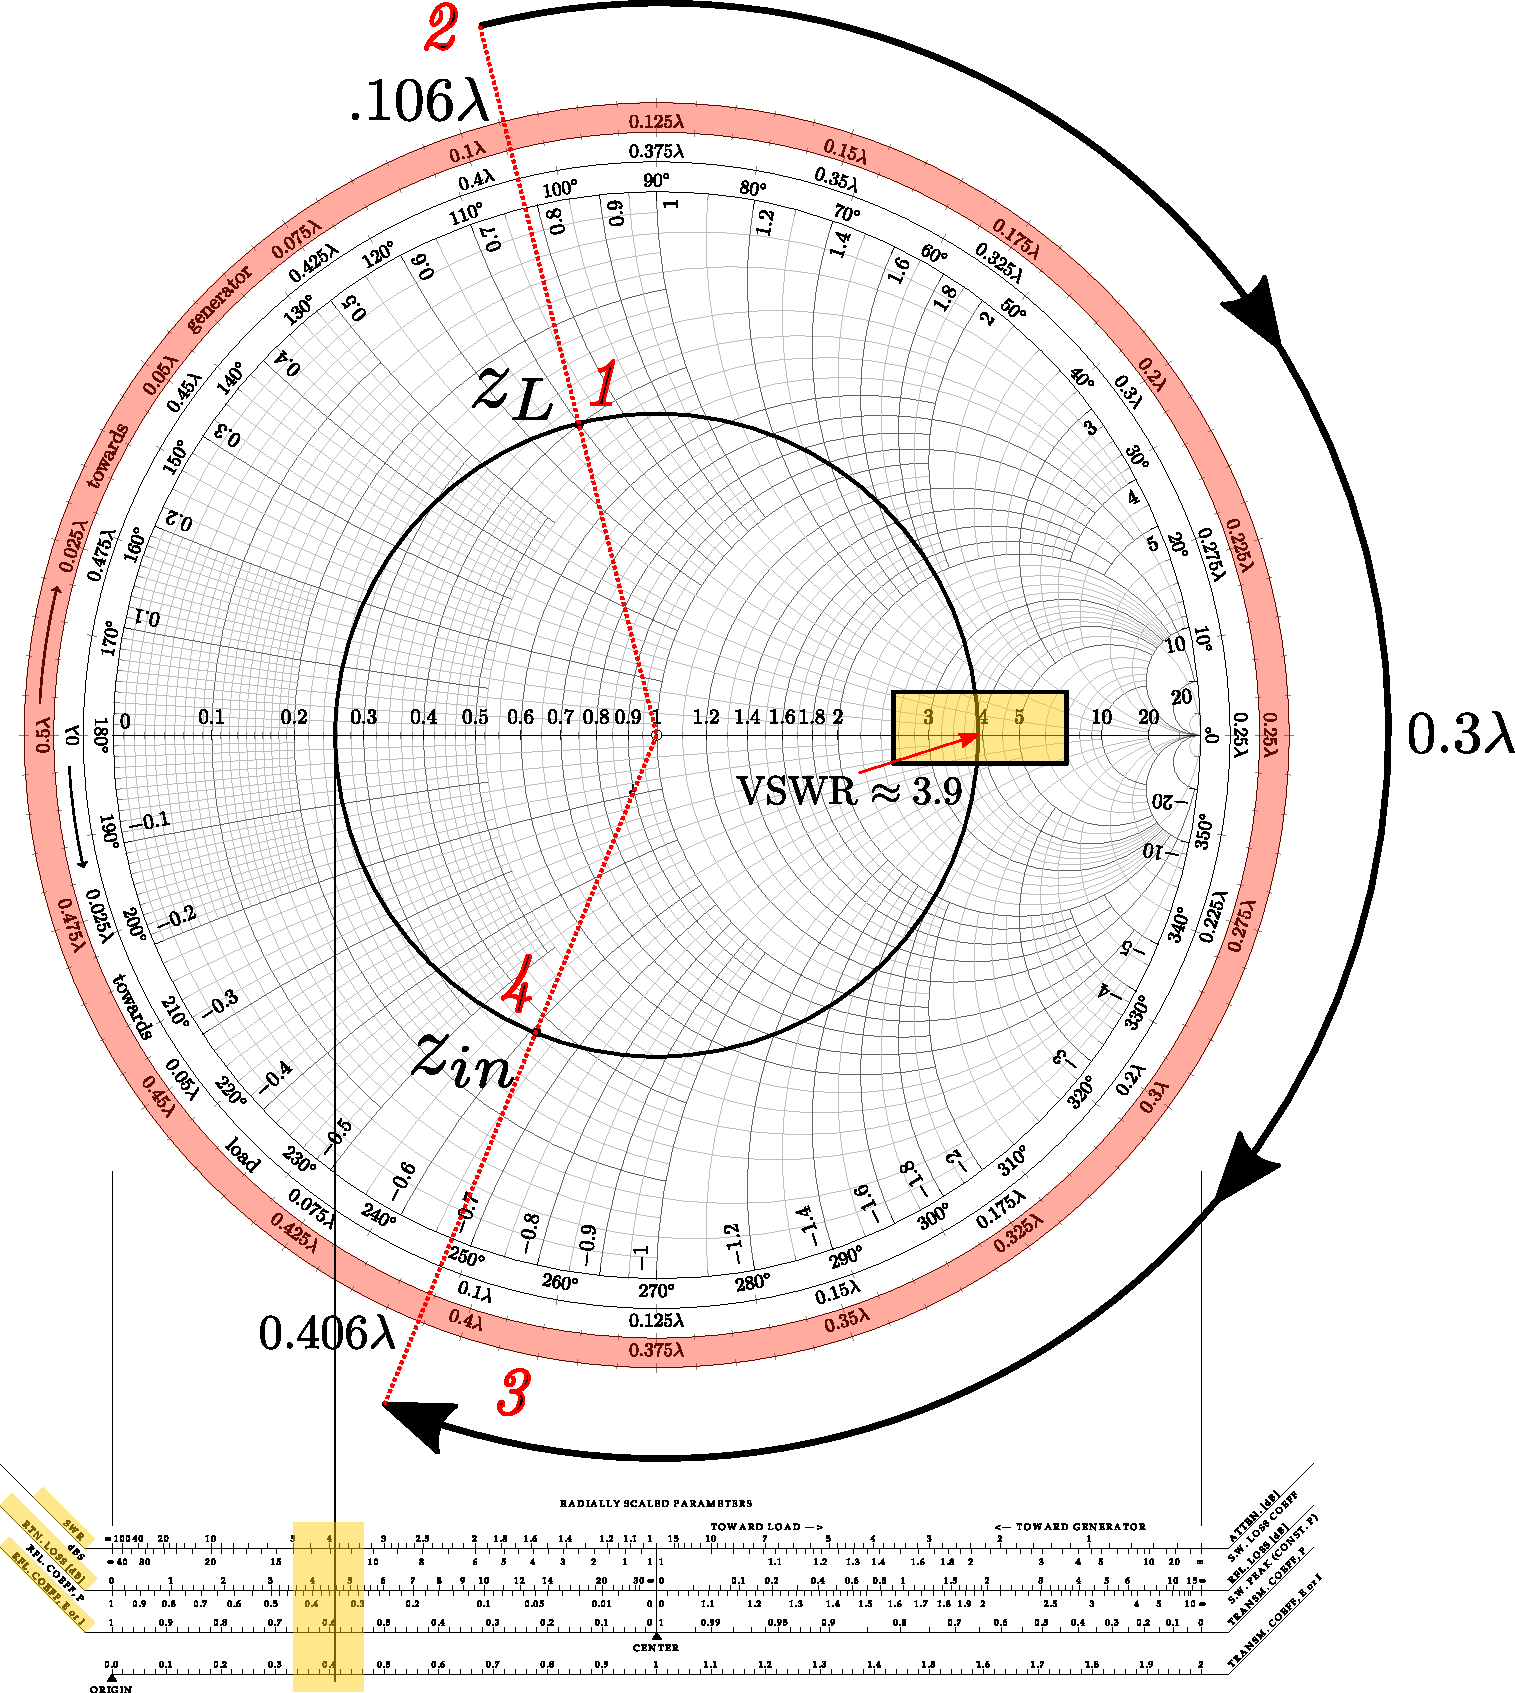
\includegraphics[width=.50\textwidth]{smith example VSWR2.pdf}
    \end{figure}
    \begin{outline}
        \1 Some Smith charts provide radially scaled parameters at the bottom of the sheet.
        \1 By drawing a vertical line from the left of the circle to the bottom, we can then read off the different values.
    \end{outline}
\end{frame}


\begin{frame}
    \frametitle{Using the Radial Axis Parameters}
    \begin{figure}[T!]
        \centering
        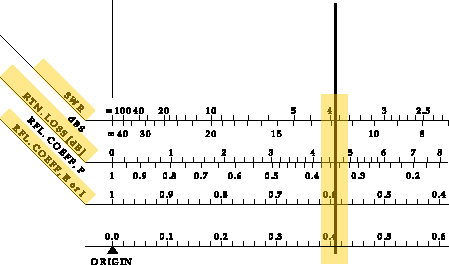
\includegraphics[width=.9\textwidth]{radial axis.pdf}
    \end{figure}
    \begin{outline}
        \1 Reading from the scales, we get, VSWR $\approx 3.9$, $|\Gamma| \approx .59$, and the return loss $\approx \SI{4.6}{\dB}$
    \end{outline}

\end{frame}
\begin{frame}
    \frametitle{Finding the Reflection Coefficient}
    \begin{outline}
        \1 The ratio of the length of the line segments $l_{O - x}$ and $l_{O - SC}$ gives us $|\Gamma|$
        \1 The point on the left of the Smith chart is the short-circuit point ($r = 0, x = 0$)
    \end{outline}
    \begin{figure}[T!]
        \centering
        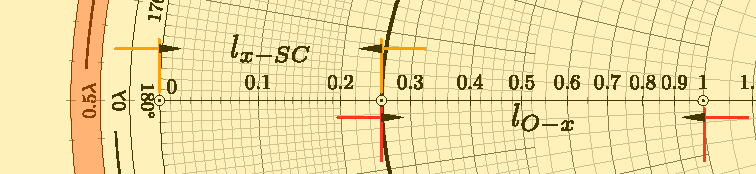
\includegraphics[width=.9\textwidth]{smith example Gamma_cropped.pdf}
    \end{figure}

\end{frame}

\begin{frame}
    \frametitle{Finding Admittance on the Smith Chart}
    \begin{columns}[T]
        \begin{column}[]{.4\textwidth}
            \begin{outline}
                \1 Admittance is just the reciprocal of the impedance
                \1 On the Smith chart, it represents the diametrically opposite point on the $|\Gamma|$-circle
                \1 For $z_L = 0.4 + \j .7$, $y_L = 1/z_L = 0.6 - \j 1.08 $
                \1 Alternatively, we can use an admittance Smith chart
            \end{outline}
        \end{column}
        \begin{column}[]{.6\textwidth}
            \begin{figure}[T!]
                \centering
                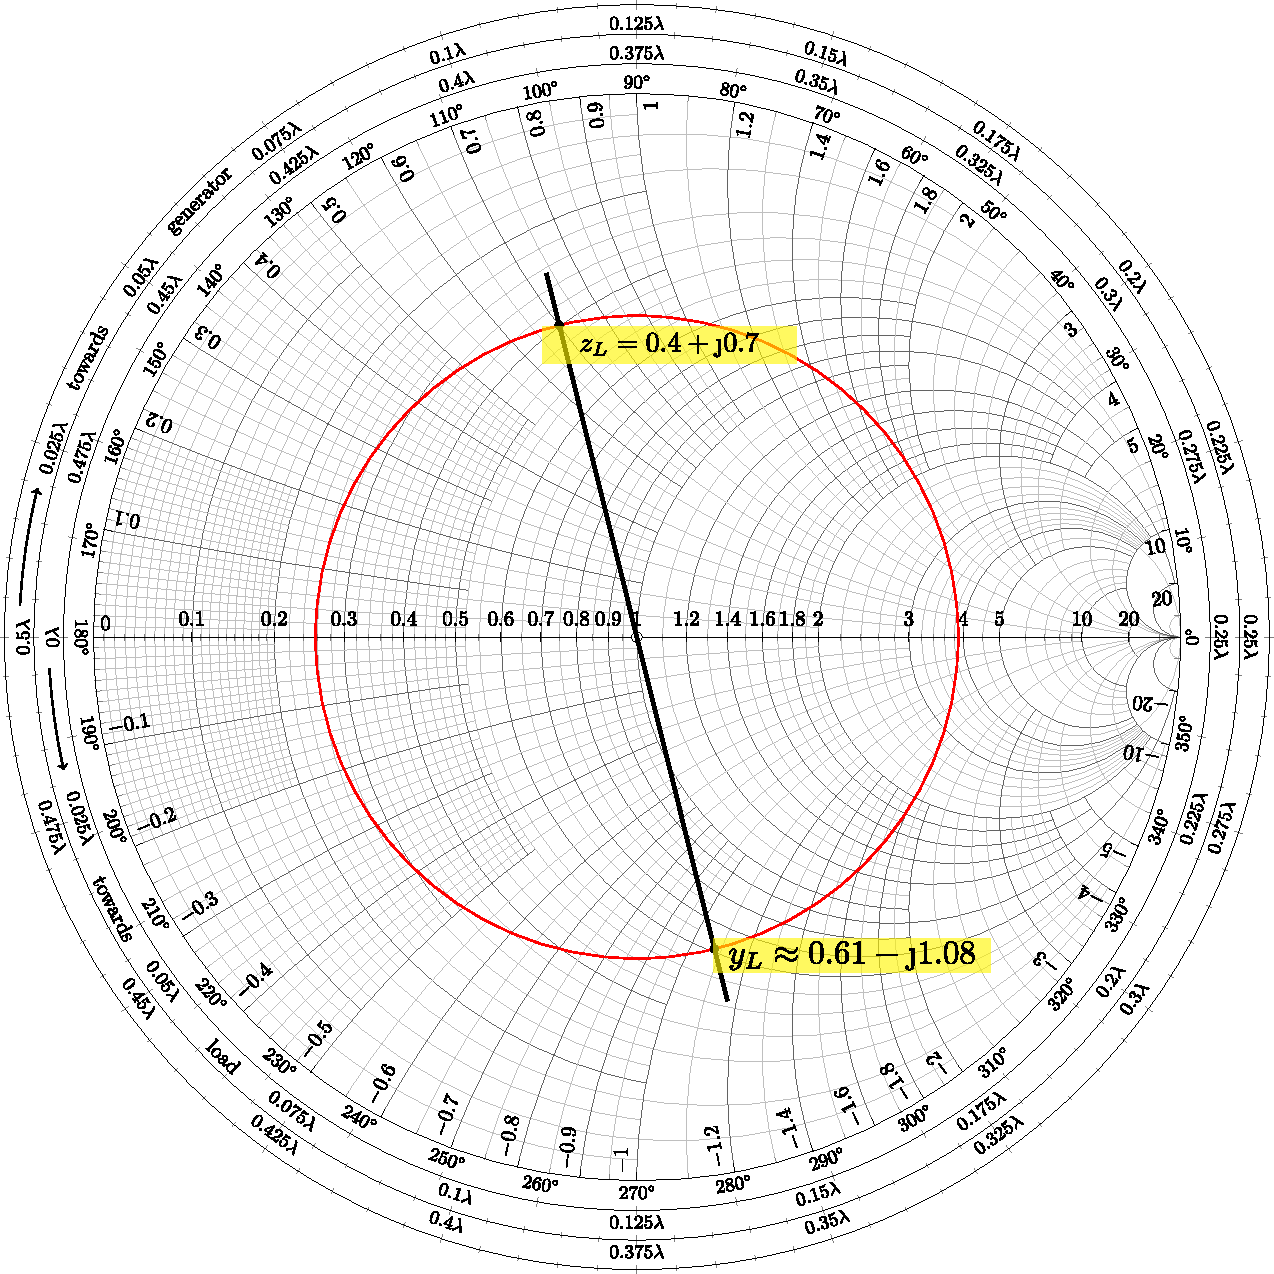
\includegraphics[width=.9\textwidth]{smith example admittance.pdf}
            \end{figure}
        \end{column}
    \end{columns}



\end{frame}



\section{Stub Matching}

\begin{frame}
    \frametitle{Stub Matching}
    \begin{columns}[T]
        \begin{column}[]{.4\textwidth}
            \begin{outline}
                \1 Stub matching introduces additional impedances/admittances in the line (often in parallel)
                \1 As parallel \textit{admittances} are added up, it is convenient to use a Smith chart showing admittance rather than impedance.
                \2 The result is a horizontally flipped admittance Smith chart.
            \end{outline}
        \end{column}
        \begin{column}[]{.6\textwidth}
            \begin{figure}[T!]
                \centering
                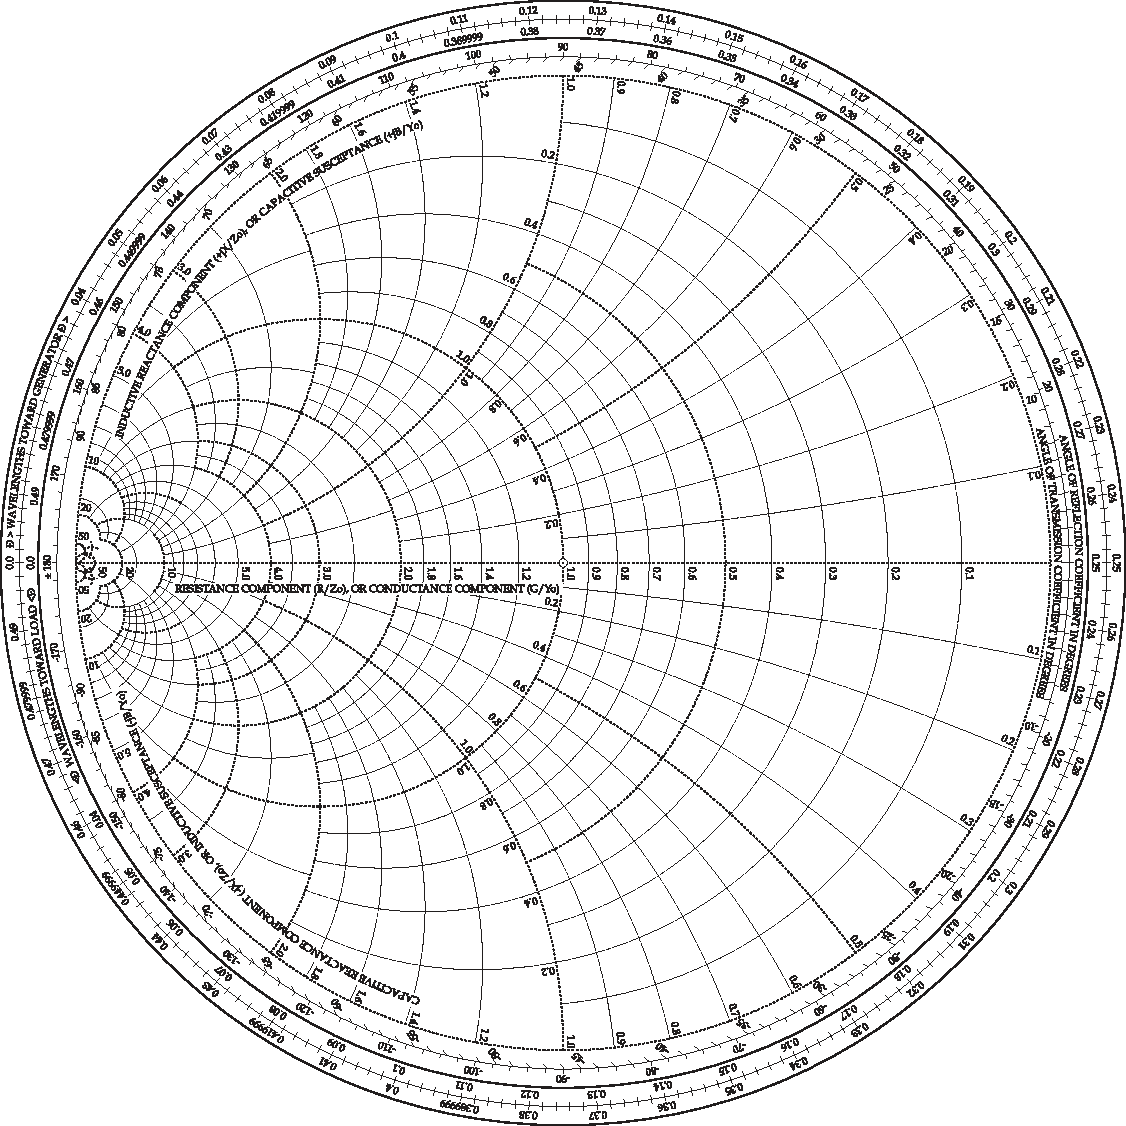
\includegraphics[width=.9\textwidth]{admittance.pdf}
            \end{figure}
        \end{column}
    \end{columns}
\end{frame}



\begin{frame}
    \frametitle{Single Stub Matching — The Problem}
    \begin{columns}[]
        \begin{column}[]{.5\textwidth}
            \begin{outline}
                \1 A short circuit stub of length $l$ is introduced in \textit{parallel} at distance $d$ from the load
                \1 As seen in the figure, we need the input impedance of the parallel combination to be $Z_0$ at the point A-A'
                \1 In other words, $y_s + y_A = y_{in} = 1$
                \1 As we are using a short circuit stub, $y_s = - \j b_A$
                \1 \textcolor{red}{The objective is to find the lengths $d$ and $l$ that generate a unity real part and zero imaginary part of admittance respectively.}
            \end{outline}
        \end{column}
        \begin{column}[]{.5\textwidth}
            \begin{figure}[]
                \centering
                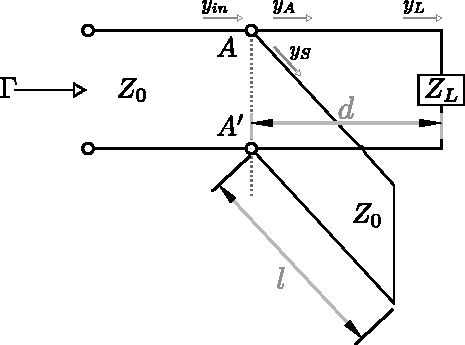
\includegraphics[width=.9\textwidth]{tline_single_stub.pdf}
            \end{figure}
        \end{column}
    \end{columns}
\end{frame}

\begin{frame}
    \frametitle{Example - Stub Matching}
    \begin{columns}[]
        \begin{column}[]{.5\textwidth}
            \begin{outline}
                \1 For a $\SI{50}{\ohm}$ transmission line connected to a load impedance $Z_L = \complexqty{35 - j 45.5}{\ohm}$
                \1 Find the position and length of the short circuit stub that matches the load to the line.
                \1 $z_L$ becomes $0.70 - \j 0.95$
            \end{outline}
        \end{column}
        \begin{column}[]{.5\textwidth}
            \begin{figure}[]
                \centering
                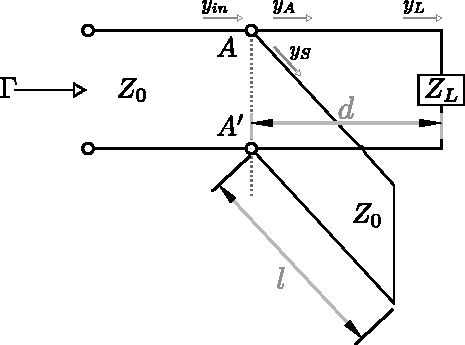
\includegraphics[width=.9\textwidth]{tline_single_stub.pdf}
            \end{figure}
        \end{column}
    \end{columns}
\end{frame}

\begin{frame}
    \frametitle{Steps for Stub Matching}
    \begin{columns}[]
        \begin{column}[]{1\textwidth}
            \begin{outline}[enumerate]
                \1 Draw $z_L$ and draw the \textcolor{red}{$|\Gamma|$-circle}
                \1 Find $y_L$ using a diametrically  opposite line
                \1 Extend the line to the perimeter and note down the \textit{wavelengths toward generator} value
                \1 Plot the \textcolor{orange}{$g =1 $} circle and note down the two points of intersection $y_{A,1} = 1 + \j b_{A,1}$ and $y_{A,2} = 1 + \j b_{A,2}$.
                \1 Find the distances $d_1$ and $d_2$ from the generator for the two points above
                \1 Find the lengths $l_1$ and $l_2$ to get the admittances $ - \j b_{A,1}$ and $ - \j b_{A,2}$
            \end{outline}
        \end{column}
    \end{columns}
\end{frame}

\begin{frame}
    \frametitle{Finding the stub distance from the load}
    \begin{figure}[]
        \centering
        \includegraphics[width=.8\textwidth]{smith  example example stub matching distance.pdf}
    \end{figure}
\end{frame}


\begin{frame}
    \frametitle{Finding the stub length from the load}
    \begin{figure}[]
        \centering
        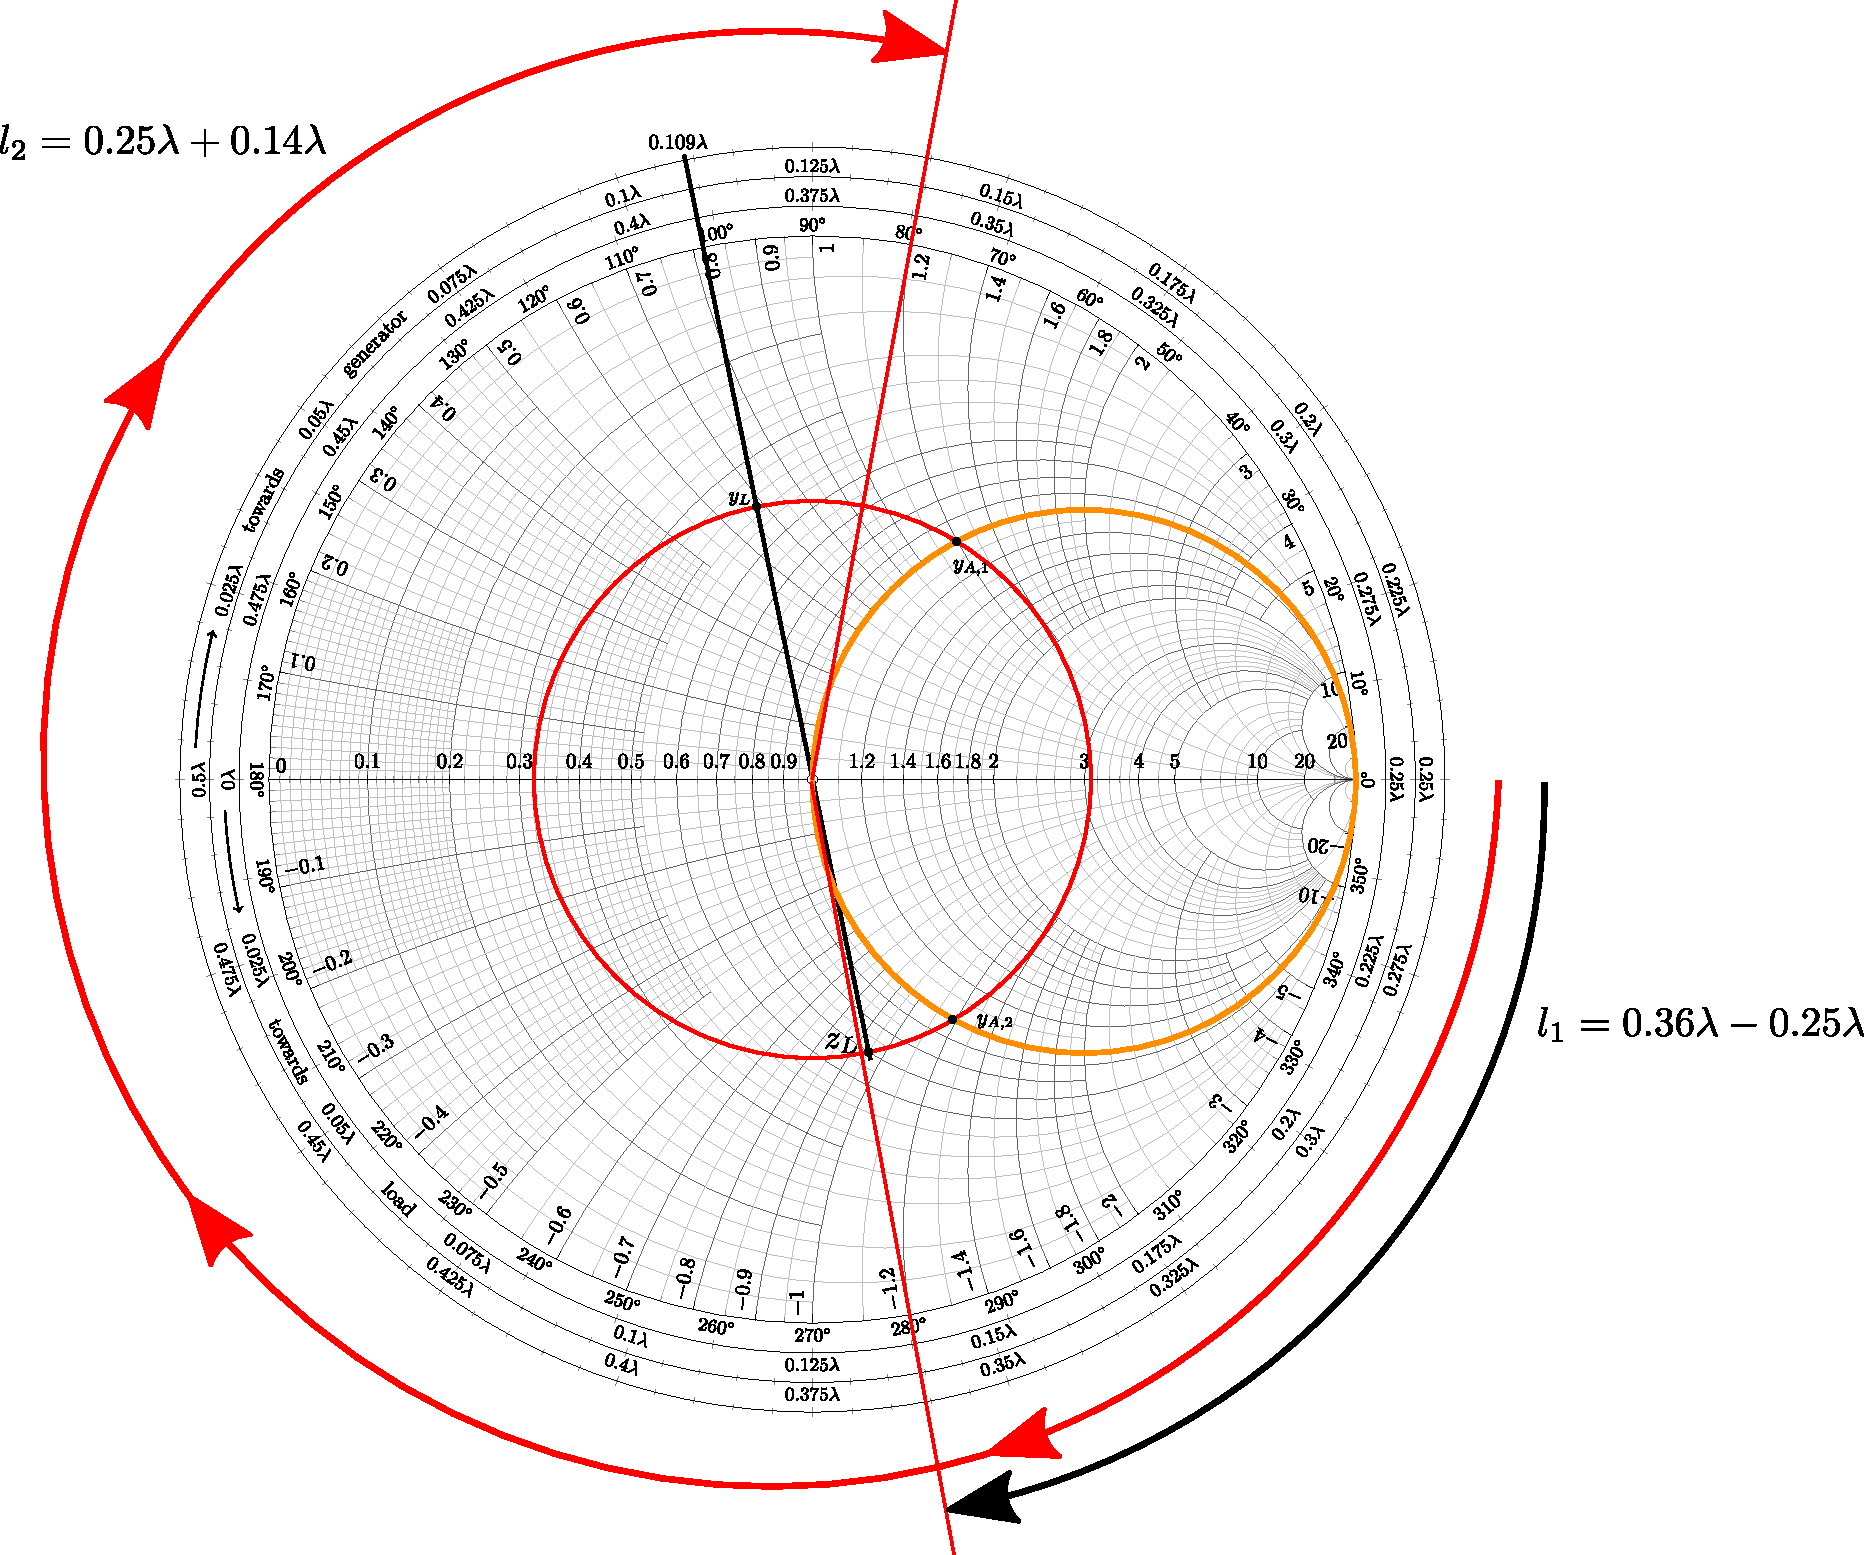
\includegraphics[width=.8\textwidth]{smith example example stub length.pdf}
    \end{figure}
\end{frame}

\begin{frame}
    \frametitle{Double Stub Matching}
    \begin{columns}[]
        \begin{column}[]{.5\textwidth}
            \begin{outline}
                \1 Single stub matching requires a precise placement of the stub from the load
                \2 This distance is a function of frequency and therefore, changes if the source frequency is changed
                \2 Also, we can't engineer the length of the stub of any given value
                \1 To avoid this and use matching at more than one frequency, we use double stub matching
            \end{outline}
        \end{column}
        \begin{column}[]{.5\textwidth}
            \begin{figure}[]
                \centering
                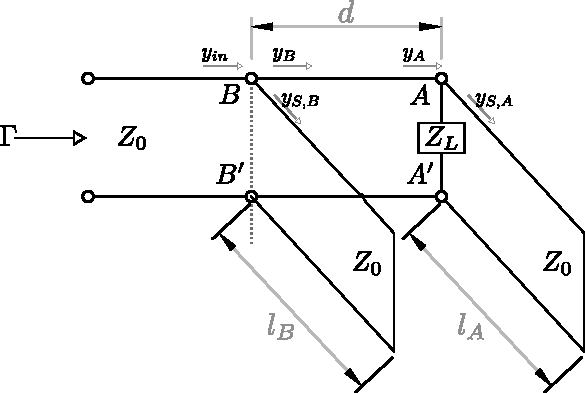
\includegraphics[width=.9\textwidth]{tline_double_stub.pdf}
            \end{figure}
        \end{column}
    \end{columns}
\end{frame}

\begin{frame}
    \frametitle{Example - Double Stub Matching}
    \begin{columns}[]
        \begin{column}[]{.5\textwidth}
            \begin{outline}
                \1 For a $\SI{50}{\ohm}$ transmission line connected to a load impedance $Z_L = \complexqty{60 + j 80}{\ohm}$
                \1 A double-stub tuner spaced $d = \lambda/8$ distance from the load for matching.
                \1 Find the lengths of the short circuit stubs that match the load to the line.
                \1 $z_L$ becomes $1.2 + \j 1.6$
                \1 $y_L$ becomes $0.3 - \j 0.40$
            \end{outline}
        \end{column}
        \begin{column}[]{.5\textwidth}
            \begin{figure}[]
                \centering
                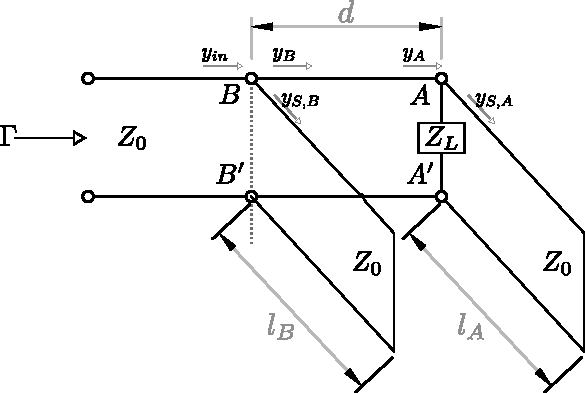
\includegraphics[width=.9\textwidth]{tline_double_stub.pdf}
            \end{figure}
        \end{column}
    \end{columns}
\end{frame}

\begin{frame}
    \frametitle{Steps for Double Stub Matching}
    \begin{columns}[]
        \begin{column}[]{1\textwidth}
            \begin{outline}[enumerate]
                \1 Plot the \textcolor{orange}{$g =1 $-circle}
                \1 Rotate the above circle by $\lambda/8$ \textit{towards the load}
                \1 Plot $y_L = 0.3 - \j 0.40$ and draw the \textcolor{green}{$g=0.3$-circle}
                \1 Mark the points $y_{A,1} = 0.30 + \j 0.30$ and $y_{A,2} = 0.30 + \j 1.75$ that are points of intersection between the \textcolor{green}{$g=0.3$-circle} and rotated \textcolor{orange}{$g=1$-circle}
                \1 The corresponding points on the \textcolor{orange}{$g=1$-circle} are $y_{B,1} = 1 + \j 1.40$ and $y_{B,2} = 1 - \j 3.50$.
            \end{outline}
        \end{column}
    \end{columns}
\end{frame}

\begin{frame}
    \frametitle{Finding the impedances}
    \begin{figure}[T!]
        \centering
        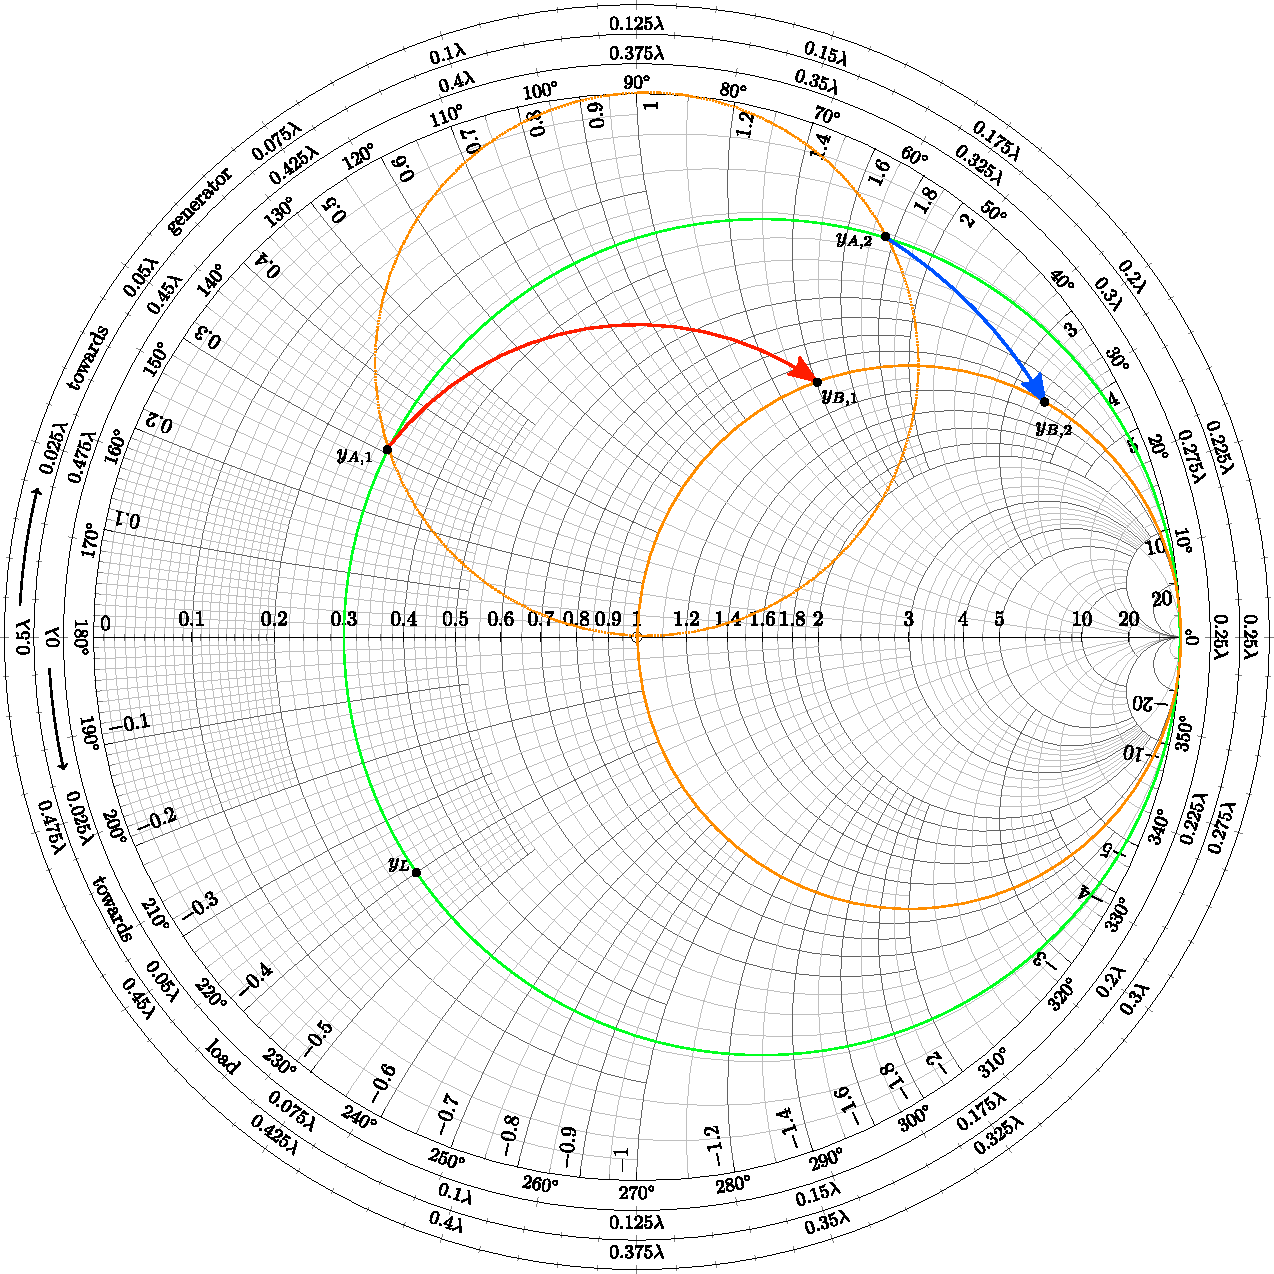
\includegraphics[width=.7\textwidth]{smith example double stub matching.pdf}
    \end{figure}
\end{frame}

\begin{frame}
    \frametitle{Finding the stub lengths}
    \begin{outline}
        \1 At the load ($A-A'$), the admittance is $y_A = y_L + y_{S,A}$
        \1 The admittances of the stub are $y_{A,1} - y_L  = 0.3 + \j 0.30 - (0.30 - \j 0.40) = \j 0.70$ and $y_{A,2} - y_L = 0.30 + \j 1.75 - (0.30 - \j 0.40) = \j 2.15$
        \1 Similarly, the admittances are simply the conjugate of $y_B$
        \1 They are $y_{B,1} = -\j 1.40$ and $y_{B,2} = -\j 3.50$
        \1 The lengths of the stub can be found in the same manner as we did for the single stub.
    \end{outline}



\end{frame}

% \end{frame}
\end{document}
